%%%%%%%%%%%%%%%%%%%%%%%%%%%%%%%%%%%%%%%%%%
% Engineering problems / LaTeX Template
%		Semester 5
%		Institut d'Optique Graduate School
%%%%%%%%%%%%%%%%%%%%%%%%%%%%%%%%%%%%%%%%%%
%	5N-OptoElec-Bloc1	/ caractérisation statique
%%%%%%%%%%%%%%%%%%%%%%%%%%%%%%%%%%%%%%%%%%
%
% Created by:
%	Julien VILLEMEJANE - 16/jul/2024
% Modified by: 06/09/24 
%	
%
%%%%%%%%%%%%%%%%%%%%%%%%%%%%%%%%%%%%%%%%%%
% Professional Newsletter Template
% LaTeX Template
% Version 1.0 (09/03/14)
%
% Created by:
% Bob Kerstetter (https://www.tug.org/texshowcase/) and extensively modified by:
% Vel (vel@latextemplates.com)
% 
% This template has been downloaded from:
% http://www.LaTeXTemplates.com
%
% License:
% CC BY-NC-SA 3.0 (http://creativecommons.org/licenses/by-nc-sa/3.0/)
%
%%%%%%%%%%%%%%%%%%%%%%%%%%%%%%%%%%%%%%%%%

\documentclass[a4paper,11pt,twoside]{book} % The default font size is 10pt; 11pt and 12pt are alternatives

\usepackage{opto_elec_villemejane}


%%%%%%%%%%%%%%%%%%%%%%%%%%%%%%%%%%%%%%%%%%%%%%%%
%%%%%%%%%%%%%%%%%%%%%%%%%%%%%%%%%%%%%%%%%%%%%%%%
%%%%%%%%%%%%%%%%%%%%%%%%%%%%%%%%%%%%%%%%%%%%%%%%
%%%%%%%%%%%%%%%%%%%%%%%%%%%%%%%%%%%%%%%%%%%%%%%%
\begin{document}
\pagestyle{empty}

\begin{minipage}[c]{.25\linewidth}
	
\includegraphics[width=4cm]{../images/Logo-LEnsE.png}
\end{minipage} \hfill
\begin{minipage}[c]{.4\linewidth}

\begin{center}
\vspace{0.3cm}
{\Large \textsc{Opto-Electronique}}

\medskip

\textbf{\Large PyCharm / Vision Industrielle (1/2)}

\end{center}
\end{minipage}\hfill

\vspace{0.5cm}

\noindent \rule{\linewidth}{1pt}
\section{Ressources}

Un \textbf{fichier archivé}, nommé \_STEP\_BY\_STEP.ZIP, regroupant l'ensemble des codes à tester au cours de la séance de découverte d'OpenCV, ainsi que les images à traiter, est à téléchargé sur le site du LEnsE : 

\textbf{Année / Première Année / Interfaçage Numérique S6 / Bloc 2 Vision Industrielle}

\vspace{0.5cm}

\begin{itemize}
	\item Téléchargez ce fichier dans un répertoire du disque dur \fbox{\textbf{U:}} de l'ordinateur.
	\item Faites un clic droit sur le fichier \textit{zip} puis \textbf{Extraire tout}. Décompressez l'archive.
\end{itemize}


\section{PyCharm / Ouvrir un projet}

Nous utiliserons le logiciel \textbf{PyCharm} pour gérer et exécuter les fichiers Python.

\begin{itemize}
	\item Lancez le logiciel \textbf{PyCharm}.
	\item Cliquez sur \fbox{\textbf{Open...}}.
	\item Sélectionnez le répertoire de travail (répertoire précédemment décompressé) puis cliquez sur \fbox{\textbf{OK}}.
\end{itemize}

Vous devriez obtenir une fenêtre de ce type :

\begin{center}
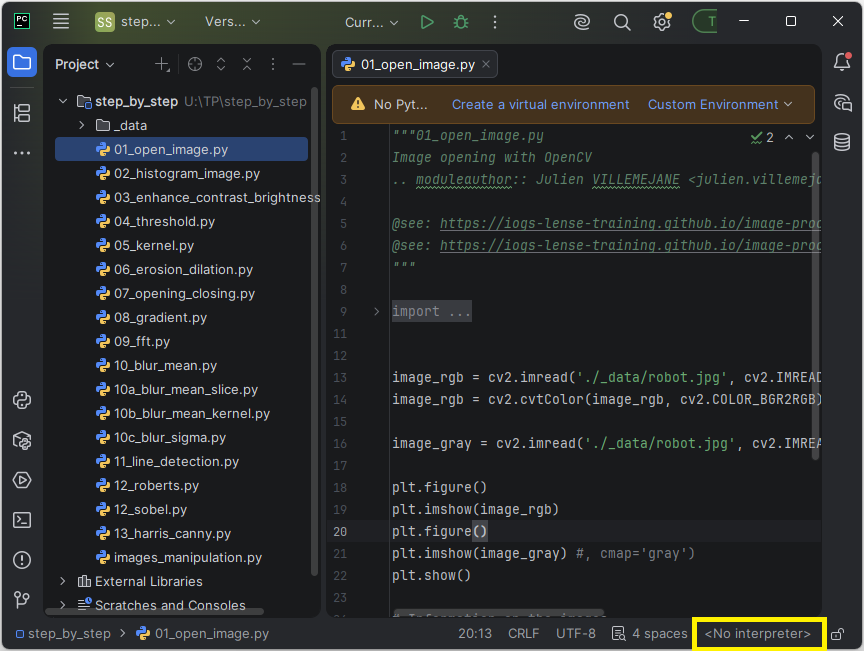
\includegraphics[width=0.7\textwidth]{pycharm_open.png}
\end{center}

Dans la partie de droite, vous avez accès à l'ensemble des fichiers que vous pouvez ouvrir en double-cliquant dessus.
	
\newpage
\section{PyCharm / Sélectionner l'interpréteur Python}

Par défaut, il n'y a pas d'interpréteur Python associé à votre projet.

\begin{itemize}
	\item Dans la zone en bas à droite de la fenêtre précédente, cliquez sur \fbox{\textbf{<No Interpreter>}}.
	\item Sélectionner ensuite \fbox{Add New Interpreter} puis \fbox{Add Local Interpreter...}
	
\end{itemize}

\begin{center}
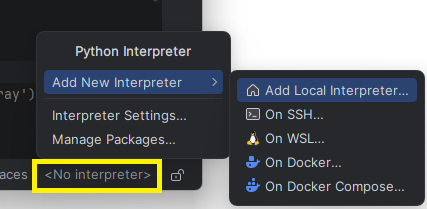
\includegraphics[width=0.4\textwidth]{pycharm_add_interpreter.png}
\end{center}

\begin{itemize}
	\item Dans le fenêtre suivante, sélectionnez \fbox{Select existing}, et dans la zone \textit{Python Path}, vérifiez que l'interpréteur \fbox{Python 3.13 - C:\textbackslash{}Program Files\textbackslash{}Python313...} est sélectionné, puis cliquez sur \fbox{\textbf{OK}}.
\end{itemize}

\begin{center}
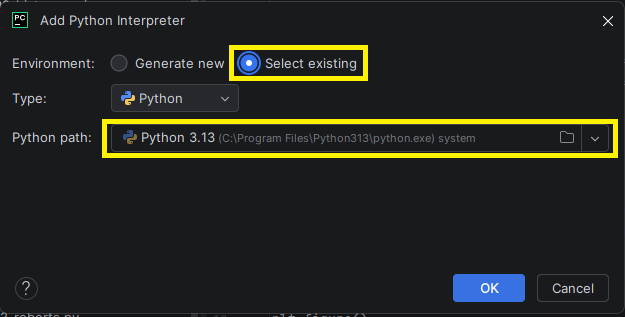
\includegraphics[width=0.6\textwidth]{pycharm_interpreter_local.png}
\end{center}


\section{PyCharm / Exécuter un script}

Pour exécuter un script Python ouvert :

\begin{itemize}
	\item Vérifiez que le fichier courant \fbox{\textit{Current file}} est sélectionné dans la barre du haut.
	\item Cliquez sur la flèche verte.
\end{itemize}

\begin{center}
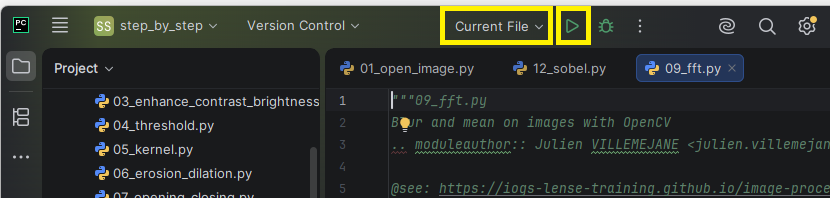
\includegraphics[width=0.7\textwidth]{pycharm_run.png}
\end{center}

\newpage
\begin{minipage}[c]{.25\linewidth}
	
\includegraphics[width=4cm]{../images/Logo-LEnsE.png}
\end{minipage} \hfill
\begin{minipage}[c]{.4\linewidth}

\begin{center}
\vspace{0.3cm}
{\Large \textsc{Opto-Electronique}}

\medskip

\textbf{\Large PyCharm / Vision Industrielle (2/2)}

\end{center}
\end{minipage}\hfill

\vspace{0.5cm}
\noindent \rule{\linewidth}{1pt}

\section{PyCharm / Images et graphiques à l'extérieur de l'interface}

Par défaut, les images et les graphiques sont affichés à l'intérieur de l'interface \textbf{PyCharm}, ce qui n'est pas forcément pratique pour agrandir ou visualiser certaines zones.

Pour paramètrer \textbf{PyCharm} afin qu'il affiche les graphiques et les images à l'extérieur de l'interface :

\begin{itemize}
	\item Cliquez sur \fbox{\textbf{File / Settings...}}.
	
\end{itemize}

\begin{center}
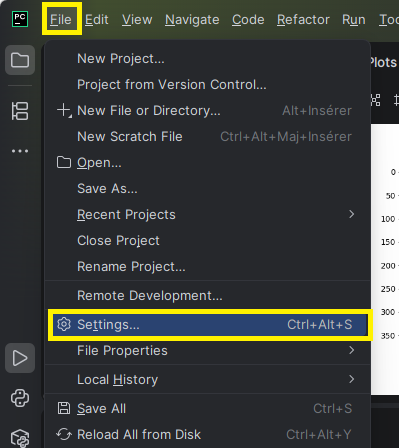
\includegraphics[width=0.4\textwidth]{pycharm_settings.png}
\end{center}



\begin{itemize}
	\item Dans la fenêtre qui s'ouvre, recherchez le terme \fbox{\textbf{plot}}.
	\item Sélectionnez l'onglet \fbox{\textbf{Python Plots}}.
	\item Décochez l'option \fbox{Show plots in tool window}.
	\item Cliquez sur \fbox{\textbf{OK}}.
\end{itemize}

\begin{center}
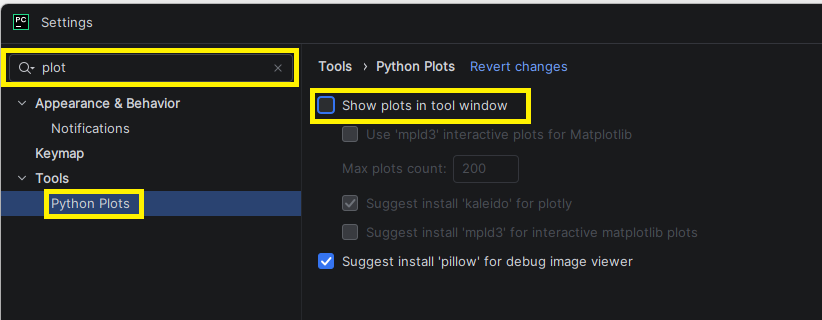
\includegraphics[width=0.8\textwidth]{pycharm_plot.png}
\end{center}

\end{document}


